\chapter{設計}
本章では,まずStuguinシステムの設計概要について述べる.
ついで,学習記録モジュール,学習記録可視化モジュールについて説明する.
そして,動機づけタイプ判定モジュールと,各タイプ向けの機能を切り替える内在化アプローチモジュールについて説明する.

\section{本システムの設計概要}
本研究では,学習に対する動機づけを内在化させるため,Stuguinシステムを提案する.
Stuguinは学習時間を記録し,その記録を可視化するiOSアプリケーションである.
本システムのシステム構成図を図~\ref{fig:system}に示す.
クライアント側は学習記録モジュール,学習記録可視化モジュール,動機づけタイプ判定モジュールおよび内在化アプローチモジュールから成る.

\begin{figure}[tb]
	\begin{center}
	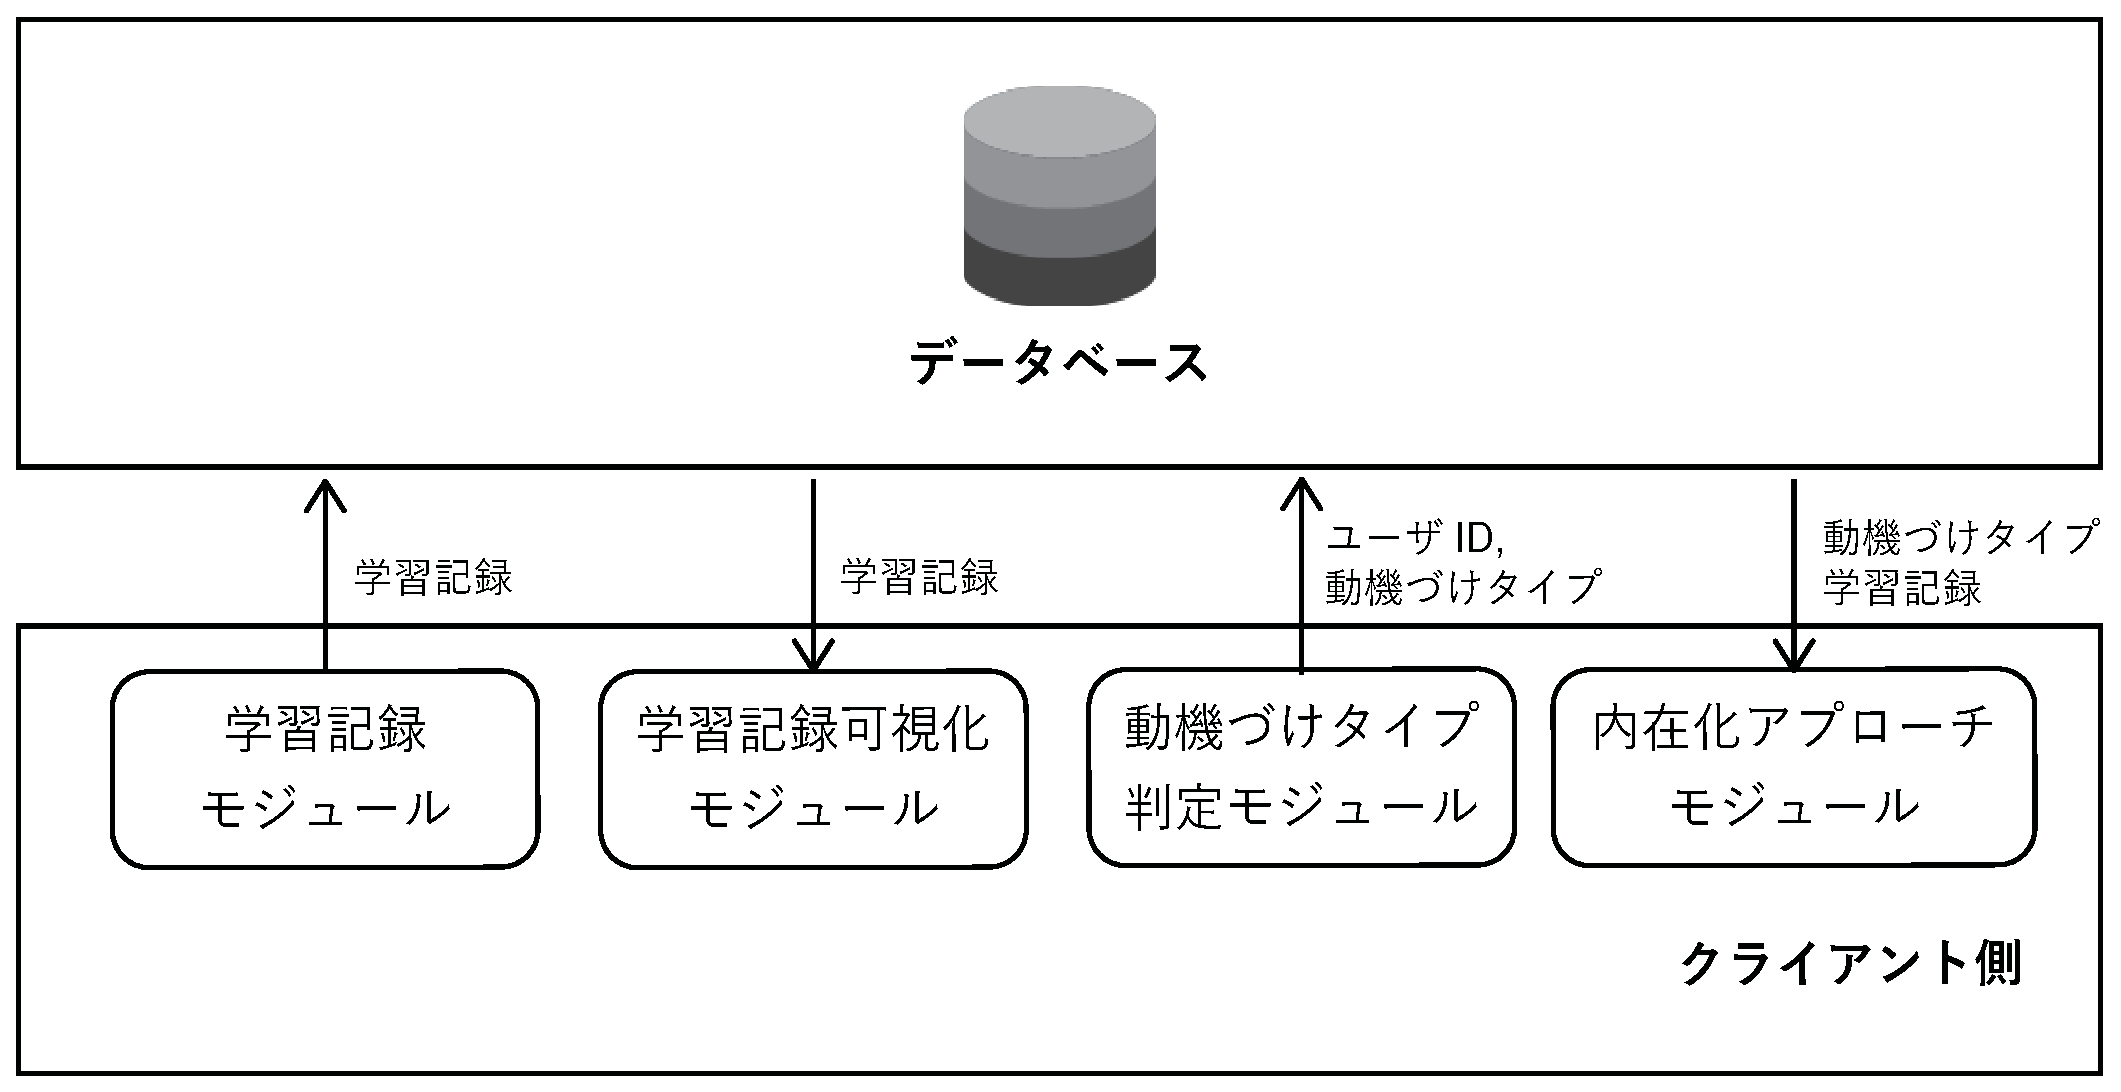
\includegraphics[width=9cm]{images/5/SystemArchitecture.eps}
	\end{center}
	\caption{システム構成図}
	\label{fig:system}
\end{figure}

\section{クライアント側設計}
本節では,クライアントであるiPhoneアプリケーションを構成する4つのモジュールについて説明する.

\subsection{学習記録モジュール}
学習記録モジュールでは,ユーザの学習時間の記録を行う.
記録には,実際に時間を測定する方法と記入する方法の2種類を用意した.
どちらの方法もまず,記録する学習の教科と内容を選択する.
実際に測定する方法では,本システムをストップウォッチのように使い学習時間を測定する.
学習時間の測定中にStuguinが閉じられた場合,学習が中断されたとみなし測定を終了する.
記入する方法では,学習を行った日時と学習時間を入力する.
記録を終了すると,サーバ側に学習記録データが保存される.

\subsection{学習記録可視化モジュール}
学習記録可視化モジュールでは,ユーザの学習記録の可視化を行う.
アプリを開いて最初に表示されるトップ画面には,過去1週間に学習した教科の割合を示す円グラフと,過去1週間の日ごとの学習時間の棒グラフが表示される.
円グラフをタップすると教科・科目の詳細画面に遷移し,それぞれの割合を1日,1週間,1ヶ月の区切りで確認することができる.
棒グラフをタップすると学習時間の詳細画面に遷移し,日ごと,週ごと,月ごとの総学習時間を確認することができる.

また,トップ画面の円グラフ・棒グラフの下には簡易的なカレンダーが表示される.
これはいくつかのマス目からなり,一番右下のマスが本日,その一つ左のマスが前日を表している.
これを用いて,過去14週間で学習を記録したマス目が色付けされて表示されるものである.

\subsection{動機づけタイプ判定モジュール}
動機づけタイプ判定モジュールは,アンケート調査を用いてユーザが抱く動機づけタイプを判定する.
アンケートには,速水らが作成した学習動機づけ尺度を利用する~\cite{hayamizu}.
このアンケートでは,回答者の動機づけが外的調整,取り入れ的調整,同一化的調整,内的調整の4つのうちどれに属するかを判定することができる.
自己決定論で定義されている動機づけと比較して無調整と統一化的調整が存在していないが,無調整は行動を全く行ったことがない状態であること,統一化的調整は内的調整とほぼ同じであることから,本尺度を利用しても問題はないと判断した.

本モジュールは1週間に一度,ユーザに対してアンケートへの回答を要求する.
このアンケートは回答必須であり,終了するまでStuguinのその他の機能を利用することはできない.
アンケート画面では質問文と,``いつも当てはまる",``しばしば当てはまる",``どちらともいえない",``めったに当てはまらない",``全く当てはまらない"の5つのボタンが表示される.
ユーザは,表示された文言に対して自身が学習を行う理由としてどの程度当てはまるかを評価する.

外的調整,取り入れ的調整,同一化的調整,内的調整に当たる記述がそれぞれ4項目ずつ,計16項目が質問される.
``いつも当てはまる"を4,``しばしば当てはまる"を3,``どちらともいえない"を2,``めったに当てはまらない"を1,``全く当てはまらない"を0として計算し,最も数値が大きかった動機づけタイプを,ユーザが現在抱く動機づけタイプと判定する.
計算結果が同点であった場合には,より外的である動機づけタイプを採用する.

判定された動機づけタイプはユーザIDとともにサーバのデータベースに保存される.

\subsection{内在化アプローチモジュール}
前項の動機づけタイプ判定モジュールにて決定された動機づけタイプから,トップ画面に表示する機能を切り替える.
用意した機能は以下の3つである.

\begin{enumerate}
  \item ポイント機能(外的調整)
  \item ランキング機能(取り入れ的調整)
  \item 目標設定機能(同一化的調整)
\end{enumerate}

括弧内は,その動機づけタイプが対象とする動機づけタイプである.
内的調整は外部からの刺激を必要としないため,対象とする機能が存在しない.

ポイント機能では1分を1ポイントとして,1週間の総学習時間をポイントに換算して表示する.
ランキング機能では1週間の総学習時間を他ユーザの分も取得し,ランキング形式で表示する.
目標設定機能でははじめに1週間の目標学習時間を設定し,以後はその目標に対する達成割合を表示する.

以上の機能のうち,ユーザの動機づけタイプと対応したもののみがトップ画面に表示される.

\section{サーバ側設計}
サーバ側では動機づけタイプに応じた処理などは行わず,データベースへの書き込み及び読み込みのみを行う.

\section{まとめ}
本章では,Stuguinシステムの設計について述べた.
次章では,本システムの実装について述べる.